\documentclass[]{article}
\usepackage[T1]{fontenc}
\usepackage{lmodern}
\usepackage{amssymb,amsmath}
\usepackage{ifxetex,ifluatex}
\usepackage{fixltx2e} % provides \textsubscript
% use upquote if available, for straight quotes in verbatim environments
\IfFileExists{upquote.sty}{\usepackage{upquote}}{}
\ifnum 0\ifxetex 1\fi\ifluatex 1\fi=0 % if pdftex
  \usepackage[utf8]{inputenc}
\else % if luatex or xelatex
  \ifxetex
    \usepackage{mathspec}
    \usepackage{xltxtra,xunicode}
  \else
    \usepackage{fontspec}
  \fi
  \defaultfontfeatures{Mapping=tex-text,Scale=MatchLowercase}
  \newcommand{\euro}{€}
\fi
% use microtype if available
\IfFileExists{microtype.sty}{\usepackage{microtype}}{}
\usepackage[margin=1in]{geometry}
\usepackage{color}
\usepackage{fancyvrb}
\newcommand{\VerbBar}{|}
\newcommand{\VERB}{\Verb[commandchars=\\\{\}]}
\DefineVerbatimEnvironment{Highlighting}{Verbatim}{commandchars=\\\{\}}
% Add ',fontsize=\small' for more characters per line
\usepackage{framed}
\definecolor{shadecolor}{RGB}{48,48,48}
\newenvironment{Shaded}{\begin{snugshade}}{\end{snugshade}}
\newcommand{\KeywordTok}[1]{\textcolor[rgb]{0.94,0.87,0.69}{{#1}}}
\newcommand{\DataTypeTok}[1]{\textcolor[rgb]{0.87,0.87,0.75}{{#1}}}
\newcommand{\DecValTok}[1]{\textcolor[rgb]{0.86,0.86,0.80}{{#1}}}
\newcommand{\BaseNTok}[1]{\textcolor[rgb]{0.86,0.64,0.64}{{#1}}}
\newcommand{\FloatTok}[1]{\textcolor[rgb]{0.75,0.75,0.82}{{#1}}}
\newcommand{\CharTok}[1]{\textcolor[rgb]{0.86,0.64,0.64}{{#1}}}
\newcommand{\StringTok}[1]{\textcolor[rgb]{0.80,0.58,0.58}{{#1}}}
\newcommand{\CommentTok}[1]{\textcolor[rgb]{0.50,0.62,0.50}{{#1}}}
\newcommand{\OtherTok}[1]{\textcolor[rgb]{0.94,0.94,0.56}{{#1}}}
\newcommand{\AlertTok}[1]{\textcolor[rgb]{1.00,0.81,0.69}{{#1}}}
\newcommand{\FunctionTok}[1]{\textcolor[rgb]{0.94,0.94,0.56}{{#1}}}
\newcommand{\RegionMarkerTok}[1]{\textcolor[rgb]{0.80,0.80,0.80}{{#1}}}
\newcommand{\ErrorTok}[1]{\textcolor[rgb]{0.76,0.75,0.62}{{#1}}}
\newcommand{\NormalTok}[1]{\textcolor[rgb]{0.80,0.80,0.80}{{#1}}}
\ifxetex
  \usepackage[setpagesize=false, % page size defined by xetex
              unicode=false, % unicode breaks when used with xetex
              xetex]{hyperref}
\else
  \usepackage[unicode=true]{hyperref}
\fi
\hypersetup{breaklinks=true,
            bookmarks=true,
            pdfauthor={Andrés Herrera Poyatos},
            pdftitle={Estructura de Datos: Práctica 1},
            colorlinks=true,
            citecolor=blue,
            urlcolor=blue,
            linkcolor=magenta,
            pdfborder={0 0 0}}
\urlstyle{same}  % don't use monospace font for urls
\setlength{\parindent}{0pt}
\setlength{\parskip}{6pt plus 2pt minus 1pt}
\setlength{\emergencystretch}{3em}  % prevent overfull lines
\setcounter{secnumdepth}{0}

\title{Estructura de Datos: Práctica 1}
\author{Andrés Herrera Poyatos}
\date{}
\usepackage{graphicx}

\begin{document}

\begin{center}
\huge Estructura de Datos: Práctica 1 \\[0.2cm]
\end{center}
\begin{center}
\large \emph{Andrés Herrera Poyatos}\\[0.1cm]
\end{center}
\normalsize


\subsection{Características del
ordenador}\label{caracteristicas-del-ordenador}

La práctica ha sido realizada en un ordenador portátil con procesador
Intel i5 a 2.5 Ghz y 8GB de memoria RAM. El sistema operativo utilizado
es Ubuntu 14.04.1 LTS mientras que el compilador es g++.

\subsection{Organización de la
práctica}\label{organizacion-de-la-practica}

Se adjunta un fichero comprimido con una carpeta para cada ejercicio.
Cada ejercicio se organiza como sigue:

\begin{itemize}
\itemsep1pt\parskip0pt\parsep0pt
\item
  Código \textbf{.cpp} del algoritmo en cuestión.
\item
  Script de bash \textbf{ejecuciones.sh} que ejecuta un programa dado un
  número de veces indicado en el script. Además, genera un archivo .dat
  con los datos obtenidos en la ejecución.
\item
  Carpeta \textbf{Datos} donde se almacenan los archivos .dat generados.
  Contiene una subcarpeta Trabajo con los datos utilizados en el
  trabajo.
\item
  Script de bash \textbf{plot.sh} con el que se crea una imagen para los
  datos obtenidos utilizando gnuplot.
\item
  Carpeta \textbf{Imagenes} donde se almacenan las imágenes .png
  generados por plot.sh. Contiene una subcarpeta Trabajo con las
  imágenes utilizadas en el trabajo.
\item
  Script de bash \textbf{ejecutar\_ejercicio\_i.sh} desde el cual se
  genera el ejecutable con el algoritmo, llama a ejecuciones.sh para su
  correspondiente ejecución y creación del fichero .dat y posteriormente
  llama a plot.sh para generar la imagen correspondiente.
\end{itemize}

Cada ejercicio tiene su apartado en el pdf con su corresponiente
enunciado y solución.

\textbf{\emph{Nota:}} Se ha utilizado el shell bash en lugar de C-shell.

\subsection{Ejercicio 1: Ordenación de la
burbuja}\label{ejercicio-1-ordenacion-de-la-burbuja}

El siguiente código realiza la ordenación mediante el algoritmo de la
burbuja:

\begin{Shaded}
\begin{Highlighting}[]
\DataTypeTok{void} \NormalTok{ordenar(}\DataTypeTok{int} \NormalTok{*v, }\DataTypeTok{int} \NormalTok{n) \{}
    \KeywordTok{for} \NormalTok{(}\DataTypeTok{int} \NormalTok{i=}\DecValTok{0}\NormalTok{; i<n}\DecValTok{-1}\NormalTok{; i++)}
        \KeywordTok{for} \NormalTok{(}\DataTypeTok{int} \NormalTok{j=}\DecValTok{0}\NormalTok{; j<n-i}\DecValTok{-1}\NormalTok{; j++)}
            \KeywordTok{if} \NormalTok{(v[j]>v[j}\DecValTok{+1}\NormalTok{]) \{}
                \DataTypeTok{int} \NormalTok{aux = v[j];}
                \NormalTok{v[j] = v[j}\DecValTok{+1}\NormalTok{];}
                \NormalTok{v[j}\DecValTok{+1}\NormalTok{] = aux;}
            \NormalTok{\}}
\NormalTok{\}}
\end{Highlighting}
\end{Shaded}

Calcule la eficiencia teórica de este algoritmo. A continuación replique
el experimento que se ha hecho antes (búsqueda lineal) con este nuevo
código. Debe:

\begin{itemize}
\item
  Crear un fichero ordenacion.cpp con el programa completo para realizar
  una ejecución del algoritmo.
\item
  Crear un script ejecuciones\_ordenacion.csh en C-Shell que permite
  ejecutar varias veces el programa anterior y generar un fichero con
  los datos obtenidos.
\item
  Usar gnuplot para dibujar los datos obtenidos en el apartado previo.
\end{itemize}

Los datos deben contener tiempos de ejecución para tamaños del vector
100, 600, 1100, \ldots{}, 30000. Pruebe a dibujar superpuestas la
función con la eficiencia teórica y la empírica. ¿Qué sucede?

\subsubsection{Cálculo de la eficiencia
teórica:}\label{calculo-de-la-eficiencia-teorica}

El algoritmo de la burbuja es un algoritmo de ordenación sencillo, luego
calcularemos exactamente el número de operaciones realizadas para su
posterior exposición en una gráfica. En primer lugar, es claro que el
siguiente código se realiza en tiempo constante:

\begin{Shaded}
\begin{Highlighting}[]
\KeywordTok{if} \NormalTok{(v[j]>v[j}\DecValTok{+1}\NormalTok{]) \{ }\CommentTok{// Comparación y acceso a los elementos v[j] y v[j+1]. 3 operaciones.}
    \DataTypeTok{int} \NormalTok{aux = v[j]; }\CommentTok{// Asignación y acceso al elemento v[j]. 2 operaciones}
    \NormalTok{v[j] = v[j}\DecValTok{+1}\NormalTok{]; }\CommentTok{// Asignación y acceso a los elementos v[j] y v[j+1]. 3 operaciones.}
    \NormalTok{v[j}\DecValTok{+1}\NormalTok{] = aux; }\CommentTok{// Asignación y acceso al elemento v[j+1]. 2 operaciones}
\NormalTok{\}}
\end{Highlighting}
\end{Shaded}

En total, 10 operaciones. Por cada iteración del bucle interno se
realizan las 10 operaciones anteriores (en el peor de los casos) más la
comparación, el acceso a un vector y el incremento correspondientes, 13
operaciones en total. Por otro lado, por cada iteración del bucle
externo se realizan anlálogamente las 3 operaciones mencionadas más la
asignación j=0 junto con la ejecución del bucle interno. Se debe sumar
la asignación inicial i=0 al resultado de aunar lo anterior. Sea
$T: \mathbb{N} \rightarrow \mathbb{N}$ la función que dado el número de
datos nos proporciona el número de operaciones realizadas, utilizando lo
anterior podemos calcularla como sigue:
\[ T(n) = 1 + \sum_{i=0}^{n-1}4\sum_{j=0}^{n-i-1}13 = 1 + \sum_{i=0}^{n-1}(4+13(n-i)) = 1 + \sum_{i=0}^{n-1}4 + 13\sum_{i=0}^{n-1}(n-i)= \]
\[ 1 + 4n + 1   3\left(\sum_{i=0}^{n-1}n - \sum_{i=0}^{n-1}i\right) = 1 + 4n + 13(n^2 - \frac{n(n-1)}{2}) = 1 + 4n + 13\frac{2n^2 - n^2 + n}{2} = 1  + 13\frac{n^2 + 105n}{2} \ \forall n \in \mathbb{N} \]
De donde es claro que $T \in O(n^2)$ y \textbf{el algoritmo de la
burbuja es cuadrático}.

\subsubsection{Resultados empíricos:}\label{resultados-empiricos}

Se muestra a continuación una gráfica con los resultados obtenidos. Es
claro que la evolución del tiempo en función del número de datos se rige
bajo una ley cuadrática aunque la pendiente de la misma es suave dada la
velocidad del ordenador al ejecutar una operación.

$\centerline{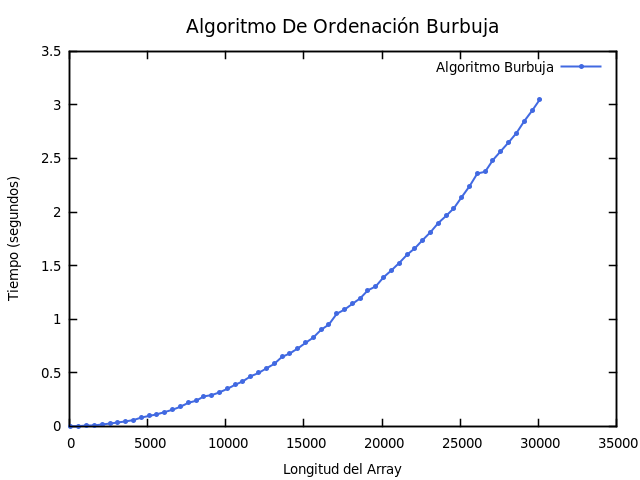
\includegraphics[height=7cm]{./Codigos/Ejercicio1/Imagenes/Trabajo/AlgoritmoBurbuja.png}}$

Si dibujamos la función obtenida para la eficiencia teórica con gnuplot
se ve claramente la parábola característica de un algoritmo cuadrático.
La forma de las dos imágenes presentadas es prácticamente equivalente.
La única diferencia es el factor de conversión de operaciones a segundos
más el tiempo utilizado por el sistema operativo en aspectos que no
tienen que ver con la ejecución del algoritmo.

\[ \centerline{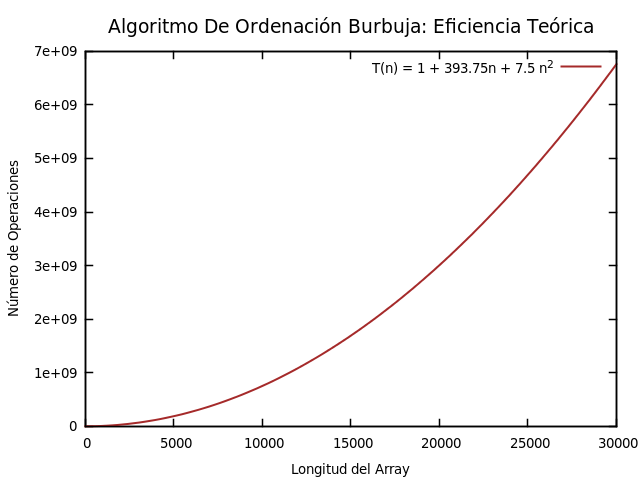
\includegraphics[height=7cm]{./Codigos/Ejercicio1/Imagenes/Trabajo/EficienciaTeorica.png}} \]

\begin{center}\rule{3in}{0.4pt}\end{center}

\subsection{Ejercicio 2: Ajuste en la ordenación de la
burbuja}\label{ejercicio-2-ajuste-en-la-ordenacion-de-la-burbuja}

Replique el experimento de ajuste por regresión a los resultados
obtenidos en el ejercicio 1 que calculaba la eficiencia del algoritmo de
ordenación de la burbuja. Para ello considere que $f(x)$ es de la forma
$ax^2+bx+c$.

\subsubsection{Resultados:}\label{resultados}

A continuación se muestra la regresión cuadrática calculada frente a los
datos obtenidos.

$\centerline{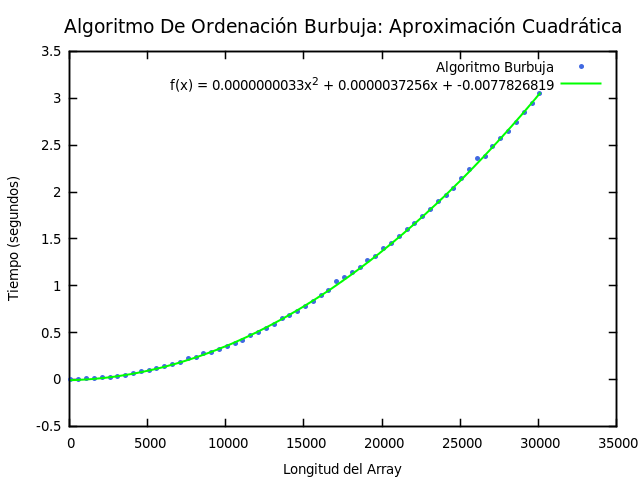
\includegraphics[height=7cm]{./Codigos/Ejercicio2/Imagenes/Trabajo/AlgoritmoBurbuja.png}}$

La \textbf{desviación media} del ajuste cuadrático responde a:
\[ \sqrt{\frac{\sum_{i=1}^{n}(y_i - f(x_i))^2}{n}} = 0.0138602 \] Como
vemos esta es mínima en relación con los valores de tiempo presentados
en la ejecución. El algoritmo burbuja implementado presenta un
comportamiento prácticamente constante pues la única posible variación
en el número de operaciones realizadas consiste en el número de veces
que se entre en el if, en cuyo caso se realiza un intercambio entre dos
componentes del vector. Por ello en la gráfica el ajuste prácticamente
coincide con casi todos los puntos.

\subsection{Ejercicio 3: Problemas de
precisión}\label{ejercicio-3-problemas-de-precision}

Junto con este guión se le ha suministrado un fichero
ejercicio\_desc.cpp. En él se ha implementado un algoritmo. Se pide que:

\begin{itemize}
\itemsep1pt\parskip0pt\parsep0pt
\item
  Explique qué hace este algoritmo.
\item
  Calcule su eficiencia teórica.
\item
  Calcule su eficiencia empírica.
\end{itemize}

Si visualiza la eficiencia empírica debería notar algo anormal.
Explíquelo y proponga una solución. Compruebe que su solución es
correcta. Una vez resuelto el problema realice la regresión para ajustar
la curva teórica a la empírica.

\subsubsection{Explicación del
algoritmo}\label{explicacion-del-algoritmo}

El algoritmo proporcionado consiste en una \textbf{busqueda binaria}
implementada de forma iterativa. La busqueda binaria permite encontrar
un elemento en un vector verificando que las componentes del mismo
mantengan una relación de orden total y que se encuentre ordenado a
través de dicha relación. En este caso se implementa el algoritmo para
un vector de enteros.

\textbf{ALGORITMO: Búsqueda Binaria}

Para cada iteración \emph{inf} representa la posición donde empieza el
subvector en el que se realiza la búsqueda y \emph{sup} la posición
donde finaliza. El proceso para cada iteración es el siguiente:

\begin{enumerate}
\def\labelenumi{\arabic{enumi}.}
\itemsep1pt\parskip0pt\parsep0pt
\item
  Se toma el elemento que se encuentra en la mitad del subvector
  \{\emph{inf}, \ldots{} , \emph{sup}\}.
\item
  Si dicho elemento es el buscado se devuelve su posición,
  $\frac{inf+sup}{2}$. En caso contrario:

  \begin{enumerate}
  \def\labelenumii{\alph{enumii})}
  \itemsep1pt\parskip0pt\parsep0pt
  \item
    Si es menor que el elemento buscado, se busca en el subvector
    \{$\frac{inf+sup}{2}+1$, \ldots{}, \emph{sup}\}.
  \item
    Si es mayor que el elemento buscado, se busca en el subvector
    \{\emph{inf}, \ldots{}, $\frac{inf+sup}{2}-1$\}.
  \end{enumerate}
\item
  Se repite el proceso hasta encontrar el valor pedido o bien cuando inf
  \textgreater{} sup, en cuyo caso el elemento a buscar no se encuentra
  en el vector y se devuelve -1.
\end{enumerate}

\subsubsection{Cálculo de la eficiencia
teórica}\label{calculo-de-la-eficiencia-teorica-1}

El peor de los casos para la búsqueda binaria es aquel en el que nunca
encuentra el elemento deseado. Sea
$T: \mathbb{N} \rightarrow \mathbb{N}$ la función tal que dado el número
de elementos del vector nos proporciona la eficiencia del algoritmo en
el caso de que no se encuentre un elemento dado. Es claro que
$T(1) = O(1)$ pues solo se comprueba dicho elemento. Para $n > 1$
podemos expresar $T$ de forma recursiva: \[ T(n) = 1 + T(n/2) \] La
explicación es sencilla, para un vector de tamaño n se realiza una
comprobación y se aplica el algoritmo en un subvector de tamaño la
mitad. Por tanto, basta resolver la anterior ecuación recurrente para
obtener la eficiencia teórica. Tomando $m = log_2 n$ se tiene que
$T(n) = T(2^m) = 1 + T(2^{m-1}) \ \forall n > 1$. Denotando
$x_m = T(2^m) \ \forall m \in \mathbb{N}$, basta resolver la siguiente
suceción recurrente:
\[ x_m = 1 + x_{m-1} \ \forall m > 0, \ x_0 = 1 \]\\El resultado de la
misma es evidente: \[ x_m = m \ \forall m \in \mathbb{N} \] Este hecho
se prueba de forma sencilla por inducción. Para $m=0$ se tiene que
$x_0 = T(2^0) = T(1) = 1$. Supesto cierto el resultado para
$m \in \mathbb{N}$ se tiene $x_{m+1} = 1 + x_m = 1 + m$ como se quería.
Volviendo a la función $T$:
\[ T(n) = T(2^m) = x_m = m = log_ 2 n \ \forall n \in \mathbb{N} \] Por
tanto, \textbf{la búsqueda binaria es un algoritmo logarítmico}.

\subsubsection{Cálculo de la eficiencia
empírica}\label{calculo-de-la-eficiencia-empirica}

Tomamos como tamaño inicial del vector 1000. Se realizan ejecuciones
desde este tamaño hasta 500000000 aumentando de 5000000 en 5000000. Si
realizamos el proceso de cálculo de la eficiencia empírica para el
código ejercicio\_desc.cpp con la búsqueda binaria se obtiene el
siguiente resultado:

$\centerline{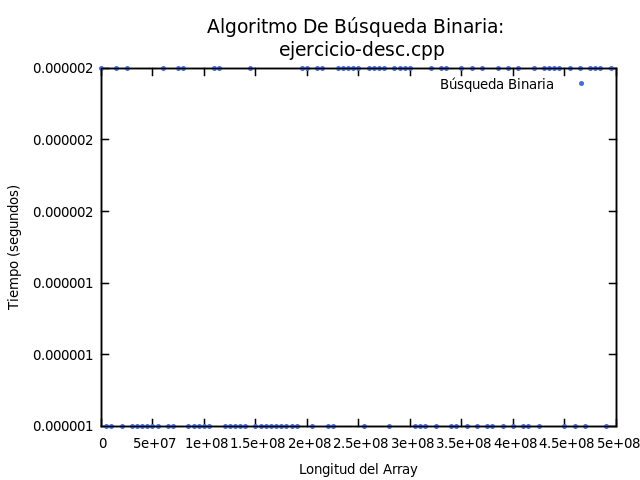
\includegraphics[height=7cm]{./Codigos/Ejercicio3/Imagenes/Trabajo/BusquedaBinaria1.png}}$

Se puede observar un valor casi nulo con una variación de $10^{-6}$. La
razón es bien sencilla: la precisión del clock de c++ es muy limitada.
Puesto que la búsqueda binaria es muy rápida por ser logarítmica, el
tiempo tomado tiende a 0 y clock no es capaz de medirlo. Para resolver
este problema he creado un nuevo código \textbf{busqueda\_binaria.cpp}
que contiene el algoritmo dado y lo ejecuta 10000 veces, calculando el
tiempo como la media de las 10000 reiteraciones. De esta forma sí se
consigue medir el tiempo con clock para las 10000 ejecuciones. Se
muestran los resultados en la siguiente imagen:

$\centerline{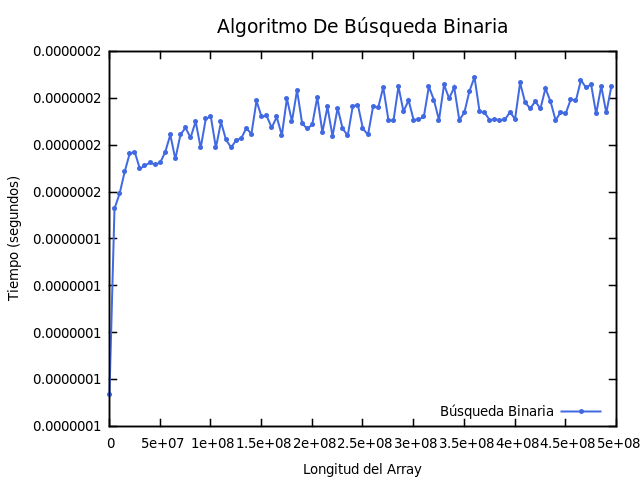
\includegraphics[height=7cm]{./Codigos/Ejercicio3/Imagenes/Trabajo/BusquedaBinaria2.png}}$

La tendencia logarítmica es clara. Si aplicamos una regresión
logarítmica a los datos se obtiene el siguiente resultado:

$\centerline{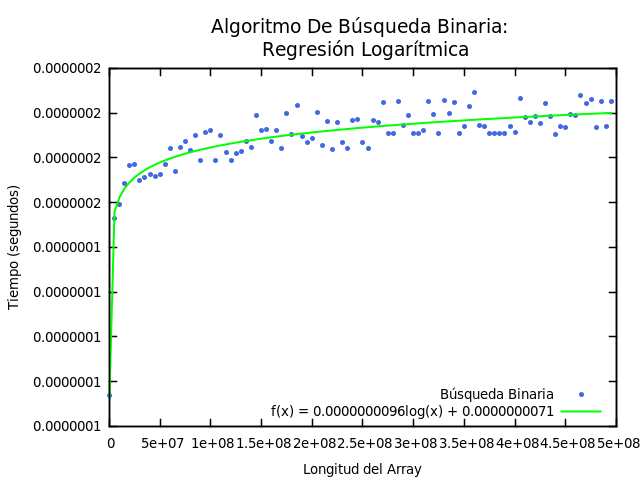
\includegraphics[height=7cm]{./Codigos/Ejercicio3/Imagenes/Trabajo/BusquedaBinariaAjuste.png}}$

En este caso la \textbf{desviación media} del ajuste logarítmico
responde a:
\[ \sqrt{\frac{\sum_{i=1}^{n}(y_i - f(x_i))^2}{n}} = 5.7476 10^{-9}\]
Siendo un valor en cierta medida importante en comparación con el valor
de los datos tomados. Esta desviación se debe al poco tiempo de
ejecución de la búsqueda binaria, lo que produce que cualquier operación
del sistema operativo afecte gravemente a los resultados.

\begin{center}\rule{3in}{0.4pt}\end{center}

\[ \pagebreak \]

\subsection{Ejercicio 4: Mejor y peor
caso}\label{ejercicio-4-mejor-y-peor-caso}

Retome el ejercicio de ordenación mediante el algoritmo de la burbuja.
Debe modificar el código que genera los datos de entrada para situarnos
en dos escenarios diferentes:

\begin{itemize}
\itemsep1pt\parskip0pt\parsep0pt
\item
  El mejor caso posible. Para este algoritmo, si la entrada es un vector
  que ya está ordenado el tiempo de cómputo es menor ya que no tiene que
  intercambiar ningún elemento.
\item
  El peor caso posible. Si la entrada es un vector ordenado en orden
  inverso estaremos en la peor situación posible ya que en cada
  iteración del bucle interno hay que hacer un intercambio.
\end{itemize}

Calcule la eficiencia empírica en ambos escenarios y compárela con el
resultado del ejercicio 1.

\subsubsection{Cálculo de la eficiencia
empírica}\label{calculo-de-la-eficiencia-empirica-1}

Nótese que de forma teórica el algoritmo sigue siendo O($n^2$) en
cualquier caso. La única variación entre los posibles casos es el hecho
de entrar o no al condicional que intercambia dos componentes del
vector. Por ello, la diferencia entre los casos no es excesiva. Se
muestra en la siguiente imagen los resultados obtenidos:

$\centerline{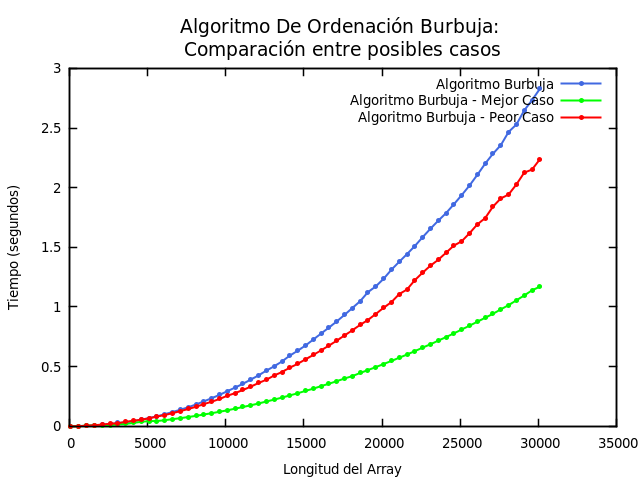
\includegraphics[height=8cm]{./Codigos/Ejercicio4/Imagenes/Trabajo/AlgoritmoBurbuja.png}}$

Es sorprendente que el supuesto peor caso obtenga mejores resultados que
un caso arbitrario. La razón es la siguiente: en el peor caso siempre se
ejecutan las mismas instrucciones pues el algoritmo siempre entra en el
bloque condicional para intercambiar dos componentes. Por tanto, durante
la ejecución del algoritmo las instrucciones que se ejecutan con el
condicional pasan a la memoria caché por su uso asiduo, librándose del
acceso a memoria ralentizaría el proceso. El caso arbitrario no sufre de
esta optimización al no ejecutarse siempre el bloque condicional. Debido
a este hecho realiza más accesos a memoria que el peor caso, obteniendo
como consecuencia los peores resultados.

\begin{center}\rule{3in}{0.4pt}\end{center}

\[ \pagebreak \]

\subsection{Ejercicio 5: Dependencia de la
implementación}\label{ejercicio-5-dependencia-de-la-implementacion}

Considere esta otra implementación del algoritmo de la burbuja:

\begin{Shaded}
\begin{Highlighting}[]
\DataTypeTok{void} \NormalTok{ordenar(}\DataTypeTok{int} \NormalTok{*v, }\DataTypeTok{int} \NormalTok{n) \{}
    \DataTypeTok{bool} \NormalTok{cambio=}\KeywordTok{true}\NormalTok{;}
    \KeywordTok{for} \NormalTok{(}\DataTypeTok{int} \NormalTok{i=}\DecValTok{0}\NormalTok{; i<n}\DecValTok{-1} \NormalTok{&& cambio; i++) \{}
        \NormalTok{cambio=}\KeywordTok{false}\NormalTok{;}
        \KeywordTok{for} \NormalTok{(}\DataTypeTok{int} \NormalTok{j=}\DecValTok{0}\NormalTok{; j<n-i}\DecValTok{-1}\NormalTok{; j++)}
            \KeywordTok{if} \NormalTok{(v[j]>v[j}\DecValTok{+1}\NormalTok{]) \{}
                \NormalTok{cambio=}\KeywordTok{true}\NormalTok{;}
                \DataTypeTok{int} \NormalTok{aux = v[j];}
                \NormalTok{v[j] = v[j}\DecValTok{+1}\NormalTok{];}
                \NormalTok{v[j}\DecValTok{+1}\NormalTok{] = aux;}
            \NormalTok{\}}
    \NormalTok{\}}
\NormalTok{\}}
\end{Highlighting}
\end{Shaded}

En ella se ha introducido una variable que permite saber si, en una de
las iteraciones del bucle externo no se ha modificado el vector. Si esto
ocurre significa que ya está ordenado y no hay que continuar. Considere
ahora la situación del mejor caso posible en la que el vector de entrada
ya está ordenado. ¿Cuál sería la eficiencia teórica en ese mejor caso?
Muestre la gráfica con la eficiencia empírica y compruebe si se ajusta a
la previsión.

\subsubsection{Cálculo de la eficiencia
teórica}\label{calculo-de-la-eficiencia-teorica-2}

Si el vector está ordenado de menor a mayor se tiene que el algoritmo de
ordenación por burbuja no realiza ningún intercambio. Por tanto, la
variable \emph{cambio} permanece siempre con el valor \emph{false} y a
la primera iteración se finaliza el algoritmo. Consecuentemente, es
claro que el algoritmo se comporta de forma lineal en el mejor caso.
Matemáticamente, realizando el mismo proceso que en el
\hyperref[Ejercicioux5cux25201:ux5cux2520Ordenaciuxf3nux5cux2520deux5cux2520laux5cux2520burbuja]{ejercicio
1}, sea $T: \mathbb{N} \rightarrow \mathbb{N}$ la función que nos
proporciona para un número de datos ordenados, $n$, el número de
operaciones que realiza el algoritmo burbuja, $T(n)$. Podemos expresar
$T(n)$ como:

\[ T(n) = 1 + 5 + 1 + \sum_{j=0}^{n}3 = 3n + 7 \]

De donde $T \in O(n)$.

\subsection{Resultados empíricos}\label{resultados-empiricos-1}

Repitiendo los experimentos con este nuevo código solo se nota una
mejoría en el mejor caso. Se adjunta un \textbf{.cpp} por cada caso
posible con los otros archivos eplicados al inicio.

En primer lugar se muestran los resultados empíricos obtenidos al
ejecutar el nuevo algoritmo para el mejor caso. Los resultados indican
una enorme mejoría en cuanto al tiempo. Además, hay severas variaciones
en la imagen tal y como pasaba con la búsqueda binaria pero de forma
menos drástica.

$\centerline{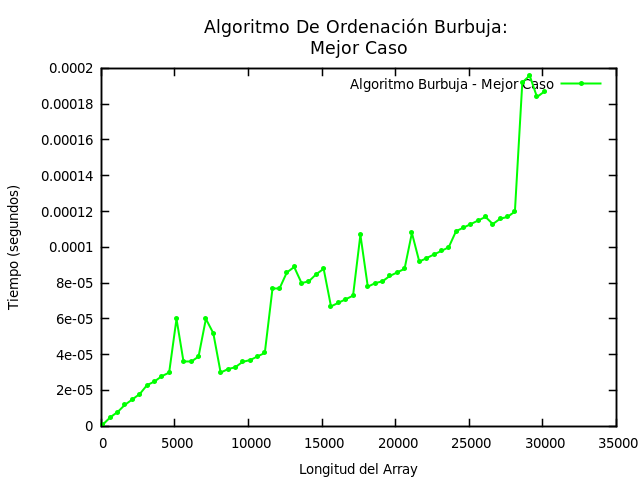
\includegraphics[height=7cm]{./Codigos/Ejercicio5/Imagenes/Trabajo/AlgoritmoBurbujaAntiguo.png}}$

Para obtener unos datos más limpios se aplica el criterio utilizado en
la búsqueda binaria que consiste en repetir una ejecución una serie de
veces y proporcionar el tiempo medio de la misma:

$\centerline{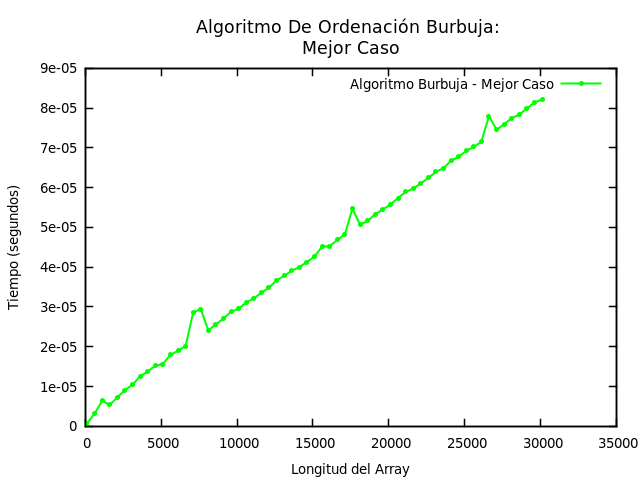
\includegraphics[height=7cm]{./Codigos/Ejercicio5/Imagenes/Trabajo/AlgoritmoBurbuja1.png}}$

El orden lineal ya es claro. Se ha reducido la varianza de los datos
como se pretendía. Con estos nuevos datos se compara el algoritmo con
peor caso y caso promedio en la siguiente imagen:

$\centerline{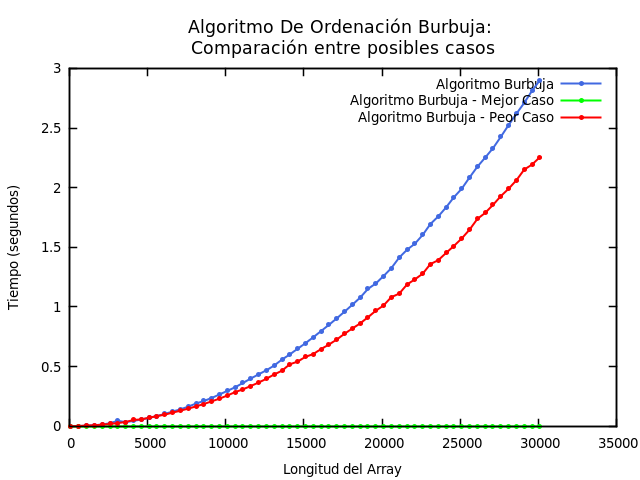
\includegraphics[height=7cm]{./Codigos/Ejercicio5/Imagenes/Trabajo/AlgoritmoBurbuja2.png}}$

Como se ve el tiempo del mejor caso se vuelve prácticamente nulo en
comparación. El peor caso sigue ganando a un caso promedio a pesar de la
optimización del algoritmo por las razones expuestas en el apartado
anterior. Cabe preguntarse si el nuevo algoritmo es mejor que el antiguo
en un caso arbitrario. El resultado de su comparación se muestra en la
siguiente imagen en la que vemos un comportamiento prácticamente similar
en ambos. El tiempo que el nuevo algoritmo gana en caso que que en
determinado momento el vector ya esté ordenado lo pierde por las
comparaciones y asignaciones extras del código.

$\centerline{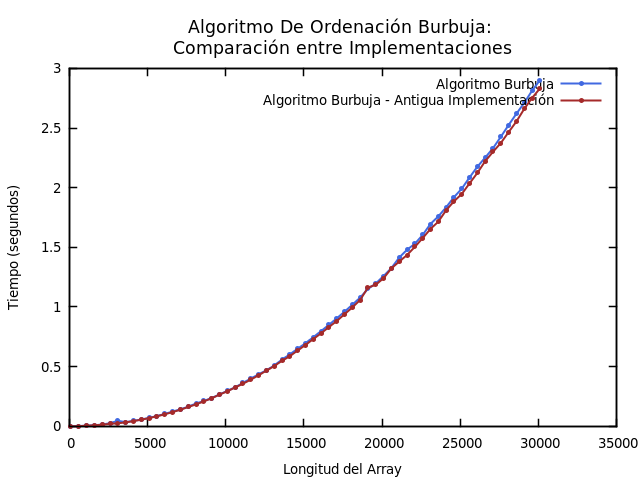
\includegraphics[height=7cm]{./Codigos/Ejercicio5/Imagenes/Trabajo/AlgoritmoBurbuja3.png}}$

\begin{center}\rule{3in}{0.4pt}\end{center}

\[ \pagebreak \]

\subsection{Ejercicio 6: Influencia del proceso de
compilación}\label{ejercicio-6-influencia-del-proceso-de-compilacion}

Retome el ejercicio de ordenación mediante el algoritmo de la burbuja.
Ahora replique dicho ejercicio pero previamente deberá compilar el
programa indicándole al compilador que optimice el código. Esto se
consigue así:

\begin{Shaded}
\begin{Highlighting}[]
\KeywordTok{g++} \NormalTok{-O3 ordenacion.cpp -o ordenacion_optimizado}
\end{Highlighting}
\end{Shaded}

Compare las curvas de eficiencia empírica para ver cómo mejora esto la
eficiencia del programa.

\subsubsection{Resultados Empíricos}\label{resultados-empiricos-2}

Se utiliza el código del \textbf{ejercicio 5} para el algoritmo de
ordenación burbuja. Los resultados obtenidos son los siguientes:

$\centerline{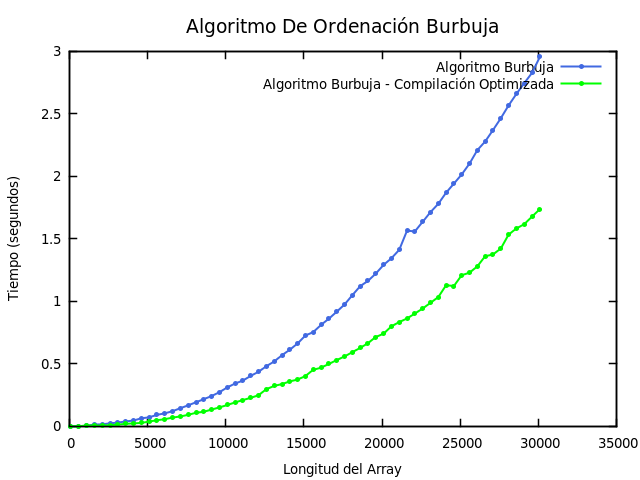
\includegraphics[height=7cm]{./Codigos/Ejercicio6/Imagenes/Trabajo/AlgoritmoBurbuja.png}}$

Es clara la amplia mejora que proporciona la optimización del código por
parte del compilador. Se obtienen tiempos que son casi la mitad con
respecto a los iniciales. Sin embargo, la optimización del código solo
afecta a la eficiencia del mismo desde el punto de vista de operaciones
por segundo, el algoritmo sigue siendo cuadrático.

\begin{center}\rule{3in}{0.4pt}\end{center}

\[ \pagebreak \]

\subsection{Ejercicio 7: Multiplicación
matricial}\label{ejercicio-7-multiplicacion-matricial}

Implemente un programa que realice la multiplicación de dos matrices
bidimensionales. Realice un análisis completo de la eficiencia tal y
como ha hecho en ejercicios anteriores de este guión.

He implementado dos algoritmos para este apartado:

\begin{itemize}
\itemsep1pt\parskip0pt\parsep0pt
\item
  Algoritmo Clásico para el producto de matrices
\item
  Algoritmo de Strassen
\end{itemize}

\subsubsection{Algoritmo Clásico para el producto de
matrices}\label{algoritmo-clasico-para-el-producto-de-matrices}

Sea $n,m,k \in \mathbb{N}$, y sean $A \in \mathbb{M}_{nxk}(\mathbb{R})$,
$B \in \mathbb{M}_{kxm}(\mathbb{R})$ dos matrices. Entonces, se define
el producto de A y B como:
\[ c_{ij} = (A.B)_{ij} = \sum_{r=1}^{k}a_{ir}.b_{rj} \ \forall i,j \in \mathbb{N} \ con \ 1 \le i \le n \ y \ 1 \le j \le m \]

Nótese que la matriz resultante $C$ pertenece a
$\mathbb{M}_{nxm}(\mathbb{R})$.

La implementación clásica del producto de matrices consiste en respetar
la definición del mismo. El código de dicha implementación se muestra a
continuación:

\begin{Shaded}
\begin{Highlighting}[]
\NormalTok{Matriz productoMatrices(Matriz A, Matriz B, }\DataTypeTok{int} \NormalTok{n, }\DataTypeTok{int} \NormalTok{k, }\DataTypeTok{int} \NormalTok{m)\{}
    \NormalTok{Matriz C(n,m);}

    \KeywordTok{for} \NormalTok{(}\DataTypeTok{int} \NormalTok{i = }\DecValTok{0}\NormalTok{; i < n; i++)\{}
        \KeywordTok{for} \NormalTok{(}\DataTypeTok{int} \NormalTok{j = }\DecValTok{0}\NormalTok{; j < m; j++)\{}
            \KeywordTok{for} \NormalTok{(}\DataTypeTok{int} \NormalTok{r = }\DecValTok{0}\NormalTok{; r < k; r++)\{}
                \NormalTok{C[i][j] += A[i][r] * B[r][j]; }\CommentTok{// Tiempo constante, O(1)}
            \NormalTok{\}}
        \NormalTok{\}}
    \NormalTok{\}}
    \KeywordTok{return} \NormalTok{C;}
\NormalTok{\}}
\end{Highlighting}
\end{Shaded}

La eficiencia del mismo es evidente. Se realizan tres bucles encadenados
con una operación constante al final del mismo. Sea
$T: \mathbb{N}x\mathbb{N}x\mathbb{N} \rightarrow \mathbb{N}$ la función
que nos proporciona para una terna de dimensiones de las matrices $A$ y
$B$, $(n,k,m)$, la eficiencia del algoritmo, $T(n,k,m)$. Podemos
expresar $T(n,k,m)$ como:

\[ T(n,k,m) =  \sum_{i=0}{n-1}\sum_{j=0}^{m-1}\sum_{r=0}{k-1}O(1) = O(n m k) \]

Por tanto , $T \in O(nmk)$. En la práctica se aplicará el algoritmo para
matrices cuadradas para poder así ver la evolución del tiempo de cómputo
en fución de su dimensión. En este caso particular es evidente que el
algoritmo resulta ser \textbf{cúbico} y por tanto su ejecución será
potencialmente inabordable para matrices de grandes dimensiones.

\subsubsection{Algoritmo de Strassen}\label{algoritmo-de-strassen}

El algoritmo de Strassen es un algoritmo recursivo para el producto de
matrices cuadradas. Fue el primer algoritmo en bajar la eficiencia
teórica del producto matricial a un orden menor que O($n^3$), en
particular, O($n^{log_{2}7}$). No solo supuso una mejoría en el cálculo
de producto de matrices de gran dimensión sino que además inicio una
investigación en torno a la búsqueda de algoritmos que mejorasen la
eficiencia obtenida a la vista de que esto era factible. Esto permitió
el descubrimiento de algoritmos como el de
\href{http://en.wikipedia.org/wiki/Coppersmith-Winograd_algorithm}{Coppersmith-Winograd}
que hacen que el producto de matrices sea una operación abordable.

El algoritmo de Strassen se basa en la siguiente obserración:

Sean $m \in \mathbb{N}$ y $n = 2^m$ una potencia de 2. Sean
$A,B \in \mathbb{M}_{nxn}(\mathbb{R})$ dos matrices cuadradas. Se puede
denotar:

\[ A = \left( \begin{array}{ccc}
a_{11} & a_{12} \\
a_{21} & a_{22} \end{array} \right) \ y
\ B = \left( \begin{array}{ccc}
b_{11} & b_{12} \\
b_{21} & b_{22} \end{array} \right)\]

Con
$a_{11}, a_{12}, a_{21}, a_{22}, b_{11}, b_{12}, b_{21}, b_{22} \in \mathbb{M}_{2^{m-1}x2^{m-1}}(\mathbb{R})$.
Definimos las matrices
$P_{1}, P_{2}, P_{3}, P_{4}, P_{5}, P_{6}, P_{7} \in \mathbb{M}_{2^{m-1}x2^{m-1}}(\mathbb{R})$
como sigue:

\begin{itemize}
\itemsep1pt\parskip0pt\parsep0pt
\item
  $P1 = (a_{11} + a_{22})(b_{11} + b_{22})$\\
\item
  $P2 = (a_{21} + a_{22})b_{11}$\\
\item
  $P3 = a_{11}(b_{12} - b_{22})$\\
\item
  $P4 = a_{22}(b_{21} - b_{12})$\\
\item
  $P5 = (a_{11} + a_{12})b_{22}$\\
\item
  $P6 = (a_{21} - a_{11})(b_{11} + b_{12})$\\
\item
  $P7 = (a_{12} - a_{22})(b_{21} + b_{22})$
\end{itemize}

Entonces se tiene que:

\[ C = A.B = \left( \begin{array}{ccc}
P_1+P_4+P_7-P_5 & P_3 + P_5 \\
\\
P_2 + P_4 & P_3 + P_1 + P_6 - P_2 \end{array} \right)\]

Nótese que las matrices $P_i$ también tienen dimenión potencia de 2.
Puesto que estas matrices se calculan mediante un producto, la misma
idea puede aplicarse a las mismas. Por tanto, el algoritmo de Strassen
sustituye productos por sumas hasta llegar a matrices con una dimensión
umbral (32 en este caso) cuyo producto sí se calcula mediante el
algoritmo clásico.

El análisis teórico del algoritmo se basa en la siguiente recurrencia:

\[ T(n) = 7T(\frac{n}{2}) + O(n^2) \]

Su obtención es sencilla. Para una matriz de dimensión \emph{n} se
calculan las matrices $P_i$ como el producto de sumas y restas de
matrices de dimensión la mitad. La operación de producto tendrá una
eficiencia de $T(\frac{n}{2})$ pues se llama recurrentemente al
algoritmo. El número 7 proviene de la realización de 7 productos
matriciales, uno por cada $P_i$. Las sumas y restas realizadas en el
proceso así como las que tienen lugar durante el cálculo de \emph{C} son
operaciones de orden de eficiencia $O(n^2)$ y el número de operaciones
es siempre constante. La suma de ambas eficiencias nos proporciona la
ecuación anterior. Para su resolución se acude al
\href{http://en.wikipedia.org/wiki/Master_theorem}{Master Theorem}
obteniendo:

\[ T(n) = n^{log_2 7} = n^{2.8074} \ \forall n \ tal \ que \ n = 2^m \ con \ m \in \mathbb{N} \]

El algoritmo expuesto requiere como entrada una matriz de dimensión
potencia de 2. Para poder aplicarlo a cualquier matriz, la idea más
sencilla es ampliar la misma con columnas y filas de ceros hasta obtener
como dimensión la siguiente potencia de 2 a la actual lo que empeora su
comportamiento y da lugar al comportamiento dado en la imagen de la
siguiente seccción.

\subsubsection{Resultados Empíricos}\label{resultados-empiricos-3}

Aunque el algoritmo de Strassen tenga una mejor eficiencia, el factor de
la misma es grande. Esto se debe a la recursividad utilizada así como a
la creación de numerosas matrices en el proceso, lo que conlleva reserva
de memoria, sumas y restas matriciales y diversas asignaciones entre
matrices. Además, el hecho de que se deba ampliar la dimensión a una
potencia de 2 produce que en realidad se multipliquen matrices de mayor
dimensión, obteniendo a veces por esta razón peores resultados que el
algoritmo clásico. Existen diversas
\href{www.cs.duke.edu/~alvy/papers/sc98/}{propuestas} para evitar este
hecho aunque todas conllevan un gran trabajo de programación.

El algoritmo clásico obtiene mejores resultados en matrices de dimensión
pequeña por las razones expuestas anteriormente. Cuando la dimensión
aumenta, el algoritmo de Strassen sí obtiene mejores resultados gracias
a su eficiencia teórica. Se muestra a continuación una comparativa entre
ambos algoritmos en la se aprecia todo lo explicado anteriormente:

$\centerline{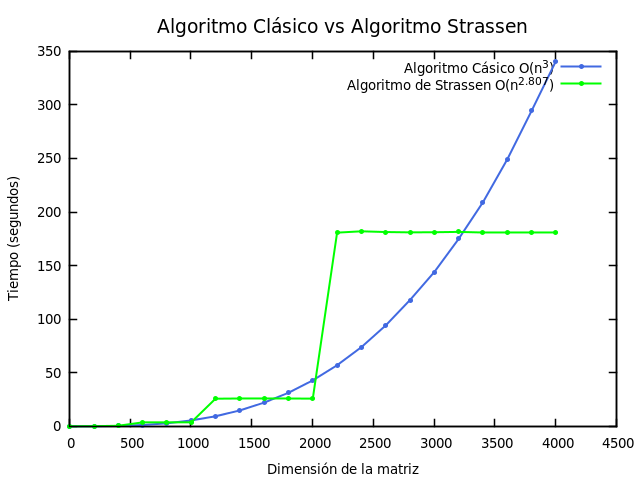
\includegraphics[height=9cm]{./Codigos/Ejercicio7/Imagenes/Trabajo/ProductoMatrices.png}}$

\begin{center}\rule{3in}{0.4pt}\end{center}

\[ \pagebreak \]

\subsection{Ejercicio 8: Ordenación por
Mezcla}\label{ejercicio-8-ordenacion-por-mezcla}

Estudie el código del algoritmo recursivo disponible en el fichero
mergesort.cpp. En él, se integran dos algoritmos de ordenación:
inserción y mezcla (o mergesort). El parámetro UMBRAL\_MS condiciona el
tamaño mínimo del vector para utilizar el algoritmo de inserción en vez
de seguir aplicando de forma recursiva el mergesort. Como ya habrá
estudiado, la eficiencia teórica del mergesort es n log(n). Realice un
análisis de la eficiencia empírica y haga el ajuste de ambas curvas.
Incluya también, para este caso, un pequeño estudio de cómo afecta el
parámetro UMBRAL\_MS a la eficiencia del algoritmo. Para ello, pruebe
distintos valores del mismo y analice los resultados obtenidos.

Se divide el ejercico en diferentes comparativas entre los algoritmos:

\begin{itemize}
\itemsep1pt\parskip0pt\parsep0pt
\item
  Algoritmo de Inserción vs Algoritmo Burbuja.
\item
  Estudio sobre UMBRAL\_MS del Mergesort.
\item
  Comparación de mergesort con otros algoritmos de ordenación O(nlog\_2
  n).
\item
  Ajuste para Mergesort e Inserción.
\end{itemize}

Se proporciona un código para cada algoritmo. Debido a las subsecciones
planteadas, en este caso se proporcionan 3 scripts
\textbf{ejecutar\_ejercico\_8\_i.sh}, uno para cada una de las 3
primeras secciones junto con un \textbf{plot\_i.sh} por script.

\subsubsection{Algoritmo de Inserción vs Algoritmo
Burbuja}\label{algoritmo-de-insercion-vs-algoritmo-burbuja}

El algoritmo de inserción utilizado en el código es un algoritmo de
ordenación de eficiencia O($n^2$) y que suele ser de los mejores con esa
eficiencia. El cálculo teórico de la misma es sencillo.

Su funcionamito se basa en el siguiente proceso:

\begin{enumerate}
\def\labelenumi{\arabic{enumi}.}
\itemsep1pt\parskip0pt\parsep0pt
\item
  Se realiza una iteración por cada elemento del vector.
\item
  Para la iteración m-ésima se presupone que se ha ordenado el subvector
  \{$1, ..., m-1$\}. Se toma el elemento en la posición m y se inserta
  en el subvector anterior manteniéndose este ordenado y con un elemento
  más.
\end{enumerate}

Es claro que cuando finalice el proceso se habrá ordenado el vector al
completo. Se muestra en la siguiente gráfica una comparativa entre este
algoritmo y el burbuja con el código del \textbf{ejercicio 5}:

$\centerline{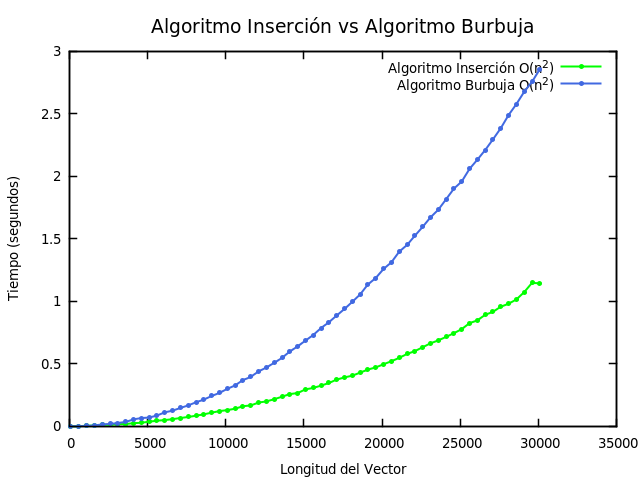
\includegraphics[height=7cm]{./Codigos/Ejercicio8/Imagenes/Trabajo/InsercionBurbuja.png}}$

El mejor factor del algoritmo de inserción con respecto al brubuja es
claro. Se debe a que el burbuja recorre todo el subvector en cada
iteración mientras que el de insercción puede parar la iteración sin
recorrer el bucle entero pues solo tiene que insertar el elemento.

\subsubsection{Estudio sobre UMBRAL\_MS del
Mergesort}\label{estudio-sobre-umbralux5fms-del-mergesort}

Se muestra en esta sección el estudio pedido sobre el parámetro
UMBRAL\_MS del mergesort. En el estudio el parámetro toma el valor 2,
20, 40, 60, 80 y 100. Se realiza la media de 1000 ejecuciones para cada
dato. Los resultados se resumen en la siguiente imagen:

$\centerline{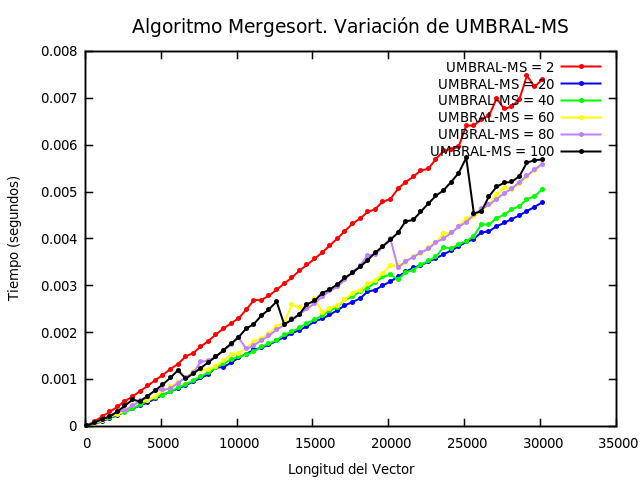
\includegraphics[height=9cm]{./Codigos/Ejercicio8/Imagenes/Trabajo/MergesortVariacion.png}}$

Se puede observar que el mejor resultado viene dado por UMBRAL\_MS=20.
Nótese que para umbrales mayores se produce un desnivel importante en
algunos puntos de la gráfica. La razón es la siguiente. Por ejemplo,
para el caso UMBRAL\_MS = 100, es claro que el algoritmo funcionará
mejor cuando las particiones del vector resulten en subvectores de
tamaño menor que 100 puesto que se aplicará inserción a vectores más
pequeños, simulando un umbral menor con su correspondiente mejoa.
Supongamos que para determinado tamaño, todas las particiones previas a
las finales tienen tamaño 101. En consecuencia, se realizará otra
partición, aplicando inserción a vectores de tamaño 50 o 51
posteriormente. En este caso se obtiene el mejor resultado posible en
términos de tiempo. Por tanto, cuando la longitud del vector está en
torno a $101 2^n$ se producirá este fenómeno, mejorando radicalmente el
tiempo del algoritmo.

Para los siguentes estudios se toma UMBRAL\_MS = 20.

\subsubsection{Comparación de mergesort con otros algoritmos de
ordenación O(nlog\_2
n)}\label{comparacion-de-mergesort-con-otros-algoritmos-de-ordenacion-onlogux5f2-n}

Se compara el mergesort con otros algoritmos de orden de eficiencia
O(nlog\_2 n). A priori, el mergesort no se suele utilizar debido a que
necesita de una segunda copia en memoria del vector para su
funcionamiento. Se comparan los resultados con:

\begin{itemize}
\itemsep1pt\parskip0pt\parsep0pt
\item
  \href{http://ronnyml.wordpress.com/2009/07/19/quicksort-en-c/}{\textbf{Quicksort:}}
  Algoritmo ampliamente utilizado y considerado uno de los mejores
  algoritmos de ordenación.
\item
  \href{https://www.youtube.com/watch?v=B7hVxCmfPtM\&index=4\&list=PLUl4u3cNGP61Oq3tWYp6V_F-5jb5L2iHb}{\textbf{Heapsort:}}
  Algoritmo basado en la estructura de datos Heap.
\item
  \href{http://www.cplusplus.com/reference/algorithm/sort/}{\textbf{Sort:}}
  Algoritmo de ordenación que proporciona c++ en el include
  \emph{algorithm}.
\end{itemize}

Los resultados obtenidos son los siguientes:

$\centerline{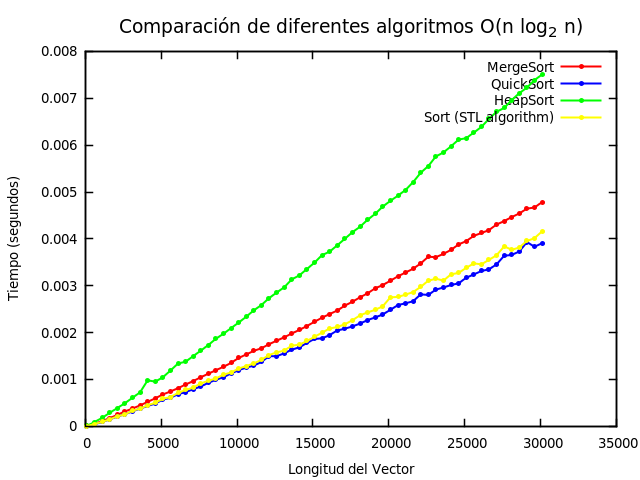
\includegraphics[height=8cm]{./Codigos/Ejercicio8/Imagenes/Trabajo/Comparacion.png}}$

Se puede apreciar que el mejor algoritmo en la práctica es el Quicksort
(recordemos que en teoría su peor caso es \textbf{cuadrático}). Obtiene
resultados similares al sort de la STL, luego presupongo que puede estar
implementado también como quicksort. Mergesort no consigue los
resultados de los dos algoritmos anteriores pero no se queda atrás. Sí
lo hace Heapsort pues a pesar de ser O($nlog_2 n$), en primer lugar crea
el heap y en segundo lugar lo ordena. Por ello obtiene tiempos dos veces
más lento.

\subsubsection{Ajustes para Inserción y
Mergesort}\label{ajustes-para-insercion-y-mergesort}

En esta sección se proporcionan los ajustes pedidos para los algoritmos
inserción y mergesort. La primera gráfica responde al primero de ellos.
Nótese la poca variación del mismo, lo que permite que el ajuste
cuadrático sea casi exacto. En este caso la \textbf{desviación media}
del ajuste cuadrático responde a:
\[ \sqrt{\frac{\sum_{i=1}^{n}(y_i - f(x_i))^2}{n}} = 0.00877017\]

$\centerline{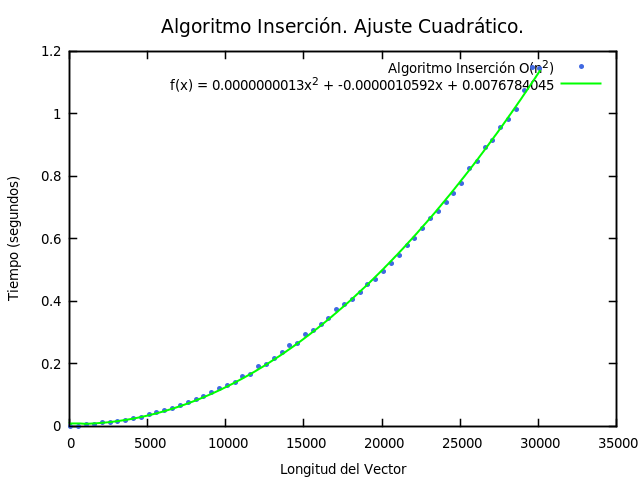
\includegraphics[height=7cm]{./Codigos/Ejercicio8/Imagenes/Trabajo/InsercionAjuste.png}}$

La siguiente imagen responde al ajuste realizado para el mergesort. Al
ser calculados los puntos como la media de 1000 ejecuciones el ajuste
tiene una \textbf{desviación media} del orden del 1\%:
\[ \sqrt{\frac{\sum_{i=1}^{n}(y_i - f(x_i))^2}{n}} = 2.86917 / 10^{-05} \]

$\centerline{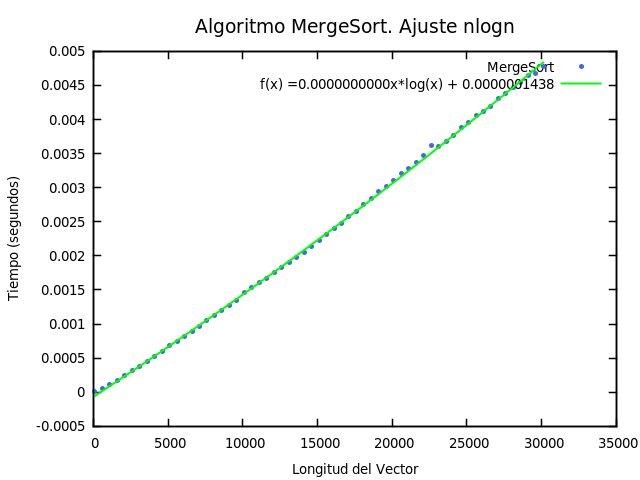
\includegraphics[height=7cm]{./Codigos/Ejercicio8/Imagenes/Trabajo/MergeSortAjuste.png}}$

En cambio, para una única ejecución se tiene una mayor dispersión de los
puntos. Esto se debe a que el ruido introducido por el sistema operativo
es significativo en relación con el tiempo que tarda el algoritmo:

$\centerline{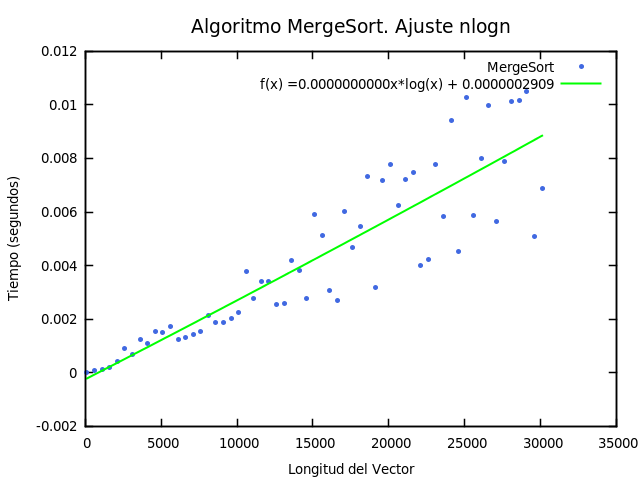
\includegraphics[height=7cm]{./Codigos/Ejercicio8/Imagenes/Trabajo/MergeSortAjuste_1.png}}$

\begin{center}\rule{3in}{0.4pt}\end{center}

\end{document}
